\chapter{Algoritmi per SpMM esistenti}
\label{ChExistingTecqs}
%----------------------------------------------------------------------------------------



\section{Notazione}	\label{notazione}
Nel seguito si utilizzerà la seguente notazione.\\
Considerando il prodotto tra 2 matrici sparse, si indicherà con $C \in \mathbb{R}^{m x n}$ il risultato del prodotto delle matrici sparse 
$A \in \mathbb{R}^{m x k},B \in \mathbb{R}^{k x n}$. Dove:\\ 
$a_{ij} \in A$ è l'elemento della riga i e colonna j della matrice A.\\
$a_{i*}~,~a_{*j}$ indicano rispettivamente la riga i-esima e la colonna j-esima della matrice A\\
$a_{i~c_z-c_w} = \left\{ a_{ij} \in a_{i*} :~ j \in [c_z,c_w] \right\}$  
indica la partizione delle colonne nel range $[c_z,c_w]$ della riga i-esima della matrice A.\\

$I_i(A)$ indica il set di indici di colonna relativi agli elementi \nnz della riga i-esima di A\\
$I^j(B)$ indica il set di indici di riga relativi agli elementi \nnz della colonna j-esima di B\\
$I(i,j)$ indica il set di indici $k$ di righe di A e di colonne di B tali che
$a_{ik}*b_{kj} \neq 0$\\
$nnz(A)$ indica il numero di non zeri della matrice A. \\ 
$nzc(A)~,~nzr(A)$ indicano rispettivamente il numero di colonne e di righe di A con almeno un elemento \nnz\\
$\hat{C}$ indica una struttura contenete risultati intermedi al prodotto $A \cdot B$.\\

\label{notazioneSp3MM}
Considerando invece il prodotto tra 3 matrici sparse, %ad esempio in applicazione di AlgebraicMultiGrid,
si indicherà con $AC_{i+1} \in \mathbb{R}^{n_{i+1} x n_{i+1} }$ il risultato del triplo prodotto tra le seguenti matrici in quest'ordine
$R \in \mathbb{R}^{n{i+1} x m} ~  AC_i \in \mathbb{R}^{n^i x n^i} ~ P \in \mathbb{R}^{m x n^{i+1}}$, dove $i~<~i+1$.\\

\label{notazioneNaming}
%TODO indici <-> indici degli elementi \nnz 
Con Sp3MM si indicherà il triplo prodotto tra matrici sparse: $AC_{i+1}=R \cdot AC_i \cdot P$
Con moltiplicazione scalare si intenderà il prodotto tra uno scalare $a \in \mathbb{R}$ per un vettore $v \in \mathbb{R}^n$\\

\section{Formulazioni SpMM}	\label{ChExistingTecqs:formulazioni}
Gli algoritmi per la risoluzione del prodotto tra due matrici sparse possono
essere classificati in base alle formulazioni e partizionamento dei dati del problema SpMM 
\cite{sysReviewChi}.\\ Le principali formulazioni del problema sono sono:
\begin{itemize}
  \item Inner-product \qquad $c_{ij} = \sum\limits_{k \in I(i,j)}  a_{ik} \ast  b_{kj}$
  \item Outer-product \qquad $C = \sum\limits_{i=1}^k  a_{*i} \otimes  b_{i*}$		
  \item row-by-row	  \qquad $c_{i*} = \sum\limits_{k \in I_i(A)}  a_{ik} \ast  b_{k*}$
  \item col-by-col    \qquad $c_{*j} = \sum\limits_{k \in I^j(B)}  a_{*k} \ast  b_{kj}$
\end{itemize}

\subsection{Rappresenzione mediante grafi}
Le formulazioni per MM possono essere rappresentate graficamente mediante
grafi a 3 strati U, W, V \cite{2dNewIdeas,cohen3LayeredGraphs} dove:
\begin{itemize}
  \item i nodi in $U \ni u_i$:   rappresentano le righe di A
  \item i nodi in $V \ni v_j$:   rappresentano le colonne di B
  \item i nodi in $W \ni w_k$:   rappresentano la dimensione in comune tra A e B
\end{itemize}
esiste un arco $(u_i,w_l) ~ \forall ~ a_{i,l} \neq 0$\\
esiste un arco $(w_l,v_j) ~ \forall ~ b_{l,j} \neq 0$\\
%%TARGET GRAPH RAPPR
Per ogni formulazione di SpMM, l'obbiettivo è quello di trovare coppie di
vertici $(u_i,v_j)$ connessi da un nodo comune $w_k$ e unire i
contributi di coppie di vertici che condividono nodi adiacenti\\ %TODO

%%INNER PRODUCT
\begin{figure}[h!]
  \centering 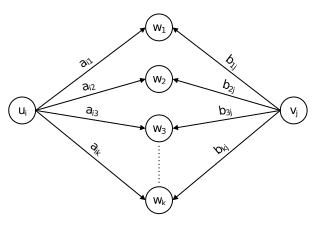
\includegraphics{layeredGraphInnerProduct.svg.png} 
  \caption[Rappresentazione grafica del calcolo di $c_{i,j}$ mediante Inner-product]
  \decoRule \label{fig:layeredGraphInnerProduct}
\end{figure}
Per la formulazione Inner-product \ref{fig:layeredGraphInnerProduct} 
è necessario esaminare ogni coppia di vertici  in U e V per trovare 
il sottoinsieme di $\tilde{W_{ij}} \subseteq W$ che connette coppie di nodi. \\
Vengono accumulati i prodotti $a_{il} \cdot b_{lj}$ relativi a $\tilde{W_{ij}}$ in $c_{ij}$.\\
È possibile osservare come la sparsità delle matrici non è sfruttata dato
che è necessario analizzare tutte le coppie di nodi $(u_i,v_j)$\\
%%OUTER PRODUCT
\begin{figure}[h!]
  \centering 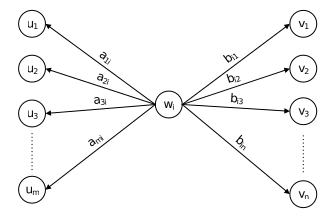
\includegraphics{layeredGraphOuterProduct.svg.png} 
  \caption[Rappresentazione grafica della componente $a_{*i} \cdot b_{i*}$ del calcolo di C mediante Outer-product]
  \decoRule \label{fig:layeredGraphOuterProduct}
\end{figure}
Per la formulazione Outer-product \ref{fig:layeredGraphOuterProduct}
è possibile identificare le coppie di vertici connesse a
partire dai nodi di W che, per matrici sufficientemente sparse,
può essere un'operazione più veloce rispetto all'Inner-product.\\
%TODO si complica l'accumulazione dei risultati intermedi
%%row-by-row
\begin{figure}[h!]
  \centering 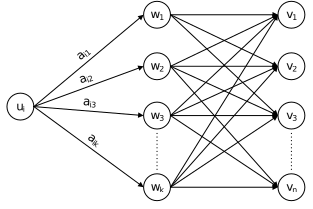
\includegraphics{layeredGraphRowByRow.svg.png} 
  \caption[Rappresentazione grafica della componente $a_{i*} \cdot B$ del 
     calcolo di C mediante formulazione row-by-row]
  \decoRule \label{fig:layeredGraphRowByRow}
  
\end{figure}
Per la formulazione Row-by-row \ref{fig:layeredGraphRowByRow}
le coppie di vertici d'interesse per il risultato di C sono identificabili 
a partire da attraversamenti del grafo indipendenti a partire dai vertici di U verso V.\\
%%col-by-col
Nel caso col-by-col vi è un attraversamento del grafo dai nodi di V a U, 
isomorfico rispetto al caso Row-by-row\\


\section{Determinazione della dimensione matrice risultante} \label{ChExistingTecqs:symbMul}
Una caratteristica comune degli algoritmi per la moltiplicazione parallela di matrici sparse è 
quella di preferire pre-allocazioni per $C$ e $\hat{C}$ 
invece di usare (ri)allocazioni dinamiche durante la computazione parallela del prodotto.\\
È possibile giustificare questa tendenza considerando genericamente algoritmi paralleli implementati con 
\label{ChExistingTecqs:openMP_for_philosophy}
direttive OpenMP come \verb|#pragma omp parallel for|, che permettono di effettuare una 
parallelizzazione di cicli, noto precedentemente il numero di iterazioni da suddividere tra i thread. \\
In questo contesto, allocazioni dinamiche richiedono la possibilità di poter uscire precedentemente dal ciclo parallelizzato
data la possibilità di fallimento di una (ri)allocazione, il che è contrario alla filosofia di parallelizzazione OpenMP
(per quanto siano disponibili costrutti per una uscita anticipata, che però richiedono una speciale configurazione, disabilitata di default per 
 motivi di performance \ref{ompSpec} )\\
Si considereranno quindi solo implementazioni per SpMM che richiedono il numero di \nnz di $C$ e $\hat{C}$ per 
effettuarne una pre-allocazione.\\

Il numero di \nnz delle righe del risultato dell'operazione di SpMM può essere determinato:\\ %%TODO bigO costs add?
sia con un UpperBound con un basso costo computazionale \\ %O(A.NZ * 2 ) accesso elemento + accesso B.IRP riga corrispondente
sia con in una modalità accurata con maggiore costo computazionale.\\ %[RBtree] || IDXMAP O(A.NZ * B.maxRowLen [* log(A.maxRowLen*B.maxRowLen)] );

\label{ChExistingTecqs:spMM_symb_num_naming}
Il calcolo (di un bound superiore) del numero di numero di \nnz di $C$ e $\hat{C}$ viene tipicamente 
denominato Prodotto Simbolico o fase simbolica, 
viceversa il calcolo effettivo dei \nnz invece Prodotto Numerico o fase numerica.\\

\subsection{UpperBound}	\label{ChExistingTecqs:symbUpperBound}
Un UpperBound sulla lunghezza di una riga risultante a SpMM è computabile come riportato nell'algoritmo 4 di \cite{sysReviewChi}.\\
In questa soluzione, ispirandosi a una formulazione row-by-row di SpMM, 
si determina la dimensione massima di ogni riga della matrice risultante come:\\
$ | I_i(C) |~\leq~\sum\limits_{ j \in I_i(A) }  | I_j(B) | $.\\
Nel caso di allocare la matrice mediante UpperBounds, è necessario effettuare anche una operazione di copia finale,
per riordinare le righe o raccoglierne i \nnz prodotti nella matrice risultate all'operazione di SpMM.\\

\subsection{Prodotto Simbolico Accurato}
L'operazione di determinare esattamente la dimensione della matrice prodotta da SpMM
è denominata in vari articoli Prodotto Simbolico e 
la seguente operazione di moltiplicazione dei vari elementi non zero è denominata Prodotto Numerico.\\

Un approccio tipico per determinare la dimensione di una riga risultante al operazione di SpMM, 
è quella di mantenere in una struttura di ricerca gli indici corrispondenti 
ai \nnz risultanti alle operazioni di prodotto, senza effettuare le costose 
operazioni di moltiplicazione floating point tra gli elementi non zero.\\
%TODO ad esempio come riportato in \ref{RITROVA ARTICOLO CHE DESCRIVE IL PRODOTTO SIMBOLICO}

\section{Algoritmi}
%%SRC STUDIES = Gustavson
Molte delle ricerche riguardo SpMM sono basate sull'algoritmo di Gustavson \cite{gustavson},
un algoritmo sequenziale basato sulla formulazione Row-by-row, riportate in forma di pseudo-codice 
in \ref{figCode:gustavsonRigheSysSurvey} e graficamente in \ref{fig:gustavsonRigheGraphicalIntel}.\\

\begin{figure}[h!]
  \caption[pseudo-codice dell'algoritmo di Gustavson]
  \centering 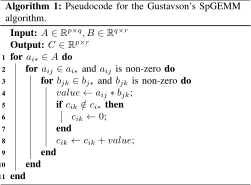
\includegraphics{gustavsonRigheSysSurvey.svg.png} \decoRule
  \label{figCode:gustavsonRigheSysSurvey}
\end{figure}
\begin{figure}[h!]
  \caption[rappresentazione grafica di una iterazione dell'algoritmo di Gustavson]
  \centering 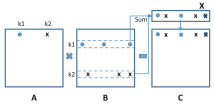
\includegraphics{gustavsonRigheGraphicalIntel.svg.png} \decoRule
  \label{fig:gustavsonRigheGraphicalIntel}
\end{figure}
È possibile notare come nell'algoritmo vi sia l'esigenza di accumulare le righe
risultanti della matrice C. Meccanismi efficienti per realizzare questa
funzionalità sono analizzati successivamente in \ref{ssec:gustavsonDerivate} %TODO FIX REF
\\


\section{Algoritmi paralleli con formulazione multidimensionale} 
Gli algoritmi paralleli risolutivi del prodotto tra matrici possono essere
classificati in base al partizionamento del carico di lavoro sui processi.\\
\begin{figure}[h!]
  \centering \includegraphics{pMM_cube.svg.png} 
  \caption[Rappresentazione grafica dell'assegnamento dei task per la risoluzione
      di SpMM in 1,2 e 3 dimensioni]\decoRule \label{fig:pMM_cube}
\end{figure}
%%WORKCUBE INTRO
L'assegnamento dei sotto problemi può essere visualizzato in un cubo di lavoro W \ref{fig:pMM_cube}
in cui ogni moltiplicazione di elementi \nnz $a_{i,k}*b_{k,j}$ è rappresentabile
con voxel $W(i,j,k)$ \cite{cartesianPartitioningModels}.
Le proiezioni $W(i,j,k)$  sulle facce del cubo relative alle matrici A e B 
hanno elementi \nnz e determinano il pattern degli elementi \nnz sulla matrice C.
%WORKCUBE NOTATIONS
\label{ChExistingTecqs:workCube}
I sottoinsiemi dei voxel di W ottenuti fissando uno o due indici sono denominati:
\begin{itemize}
  \item Layers: W(i,:,:),W(:,j,:),W(:,:,k)
  \item Fibers: Intersezioni di Layers relativi a indici diversi, e.g. W(i,j,:)
  \item Cuboid: Sottoinsiemi di W con tutte le dimensioni minori delle 
   dimensioni delle matrici corrispondenti
\end{itemize}

\subsection{Matrici ipersparse e rappresentazione DCSC}
È possibile definire una matrice sparsa A, come {\bf ipersparsa }se $nnz(A)$ è
inferiore alla sua dimensione più grande N \cite{2dNewIdeas} \\ %TODO newIdeas 14.2.2 x matrici quadrate
Tipicamente questa tipologia di matrici è rara nell'algebra lineare numerica.
Infatti, nella soluzione di sistemi lineari, le matrici sono quadrate, ed avere un numero di nonzeri inferiore alla dimensione 
vorrebbe dire che alcune equazioni non hanno coefficienti, 
il che nei problemi provenienti da equazioni differenziali chiaramente non ha senso.
Tuttsvia, questa tipologia di matrici trova applicazioni nel partizionamento di matrici sparse 
e nel processamento grafi, particolarmente se in parallelo.\\

Data una suddivisone bidimensionale di una matrice sparsa, %TODO quadrata
per un processamento parallelo in una griglia di p processi, si ha che ogni processo
verrà assegnato ad una matrice di dimensione circa $(n/\sqrt{p})~x~(n/\sqrt{p})$. %TODO ~~
L'occupazione globale di spazio di memoria sarà pari a 
$O(nnz + p \cdot n/\sqrt{p}) = O(nnz + n \cdot \sqrt{p})$ con CSC che è maggiore
dell'occupazione totale della matrice in un singolo processo $O(n + nnz)$.\\
Allo scalare del numero di processi p, il termine $n\sqrt{p}$ domina $nnz$.\\
%TODO The ineffciency of CSC leads to a more fundamental problem: any algorithm that
%uses CSC and scans all the columns is not scalable for hypersparse matrices. 
%Even without any communication at all, such an algorithm cannot scale for $n\sqrt{p} > \max{flops,nnz}$

Per queste ragioni è possibile utilizzare la rappresentazione \\
{\bf D}ouble{\bf C}ompressed{\bf S}parse{\bf C}olumns,\ref{fig:DCSCvsCSC}
che ha un'occupazione di memoria pari ad $O(nnz)$
eliminando eventuali ripetizioni nell'array di puntatori delle colonne (JC) nel formato CSC.
È possibile favorire un rapido accesso alle colonne della matrice mediante un
array ausiliario di indici delle colonne \nnz
%TODO qualche spiegazione ulteriore
\begin{figure}[h!]
  \caption[confronto delle rappresentazioni DCSC e CSC ]
  \centering 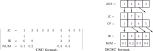
\includegraphics{DCSCvsCSC.svg.png} \label{fig:DCSCvsCSC}
\end{figure}

\subsection{Moltiplicazione tra matrici ipersparse rappresentate con DCSC}
\label{ssec:hypersparseMM}
Segue la descrizione di un algoritmo risolutivo per la moltiplicazione tra matrici
ipersparse \cite{2dNewIdeas}, basato su una formulazione outer-product ed
utilizzato in alcuni algoritmi SpMM.\\
lo pseudo-codice dell'algoritmo è riportato in \ref{figCode:hypersparseMM} 


{\bf fase di preprocessamento} \\
viene effettuata una trasposizione di B, così da avere un indicizzamento rapido delle righe di B
in formato DCSC, necessario per la
formulazione outer-product.\\ 
%costo di trasposizione varia tra $O(n + nnz(B) \to nnz(B) lg nnz(b)) in base all implementazione
Viene effettuata l'intersezione tra gli indici delle colonne non zero di A e
delle righe non zero di B, identificando così il set $Isect = A.JC \cap B^T.JC$ degli
indici che partecipano all'outer-product.\\
\\
Successivamente vengono effettuati $|Isect|$ prodotti cartesiani \ref{fig:hypersparseMMGraphical} 
generanti matrici $a_{*i} \cdot b_{i*}$, i cui elementi è possibile mettere in biiezione 
con la lista di indici $(r_{id},c_{id})$ derivante dal prodotto cartesiano tra gli indici
di riga non zero della colonna i-esima di $B^T$ e gli indici di riga non zero 
della colonna i-esima di $A$.\\
La matrice risultante C può essere ottenuta mediante l'unione di queste liste,
sommando i contributi degli elementi aventi gli stessi indici in liste
diverse.\\
Per implementare la costruzione di C dagli outer-products
è utilizzata una coda con priorità contenete elementi relativi ai
prodotti cartesiani per le colonne di $A$ e le colonne di $B^T ~\in~ Isect$, 
aventi per chiave $(r_{id},c_{id})$ e per valore il prodotto relativo e l'indice
della colonna di $A$ o $B^T$ relativa.\\
Verrà ripetutamente estratto il minimo dalla coda e reinserito
l'elemento successivo dalla lista di indici di relativa, sommando i
contributi di elementi con la stessa chiave.
I risultati verranno accumulati in uno stack mediante una rappresentazione
matriciale a coordinate degli elementi % TODO CHECK COO LIKE STACK ACCUMULATE
per poi essere convertiti nella matrice finale C in formato DCSC.\\

La complessità computazionale dell'algoritmo è $O(nzc(A) + nzr(B) +flops \cdot lg( ni))$
dove $ni$ è la dimensione della coda con priorità e $flops$ è il numero di
operazioni aritmetiche necessarie per il prodotto di A e B.\\

\begin{figure}[h!]
  \centering 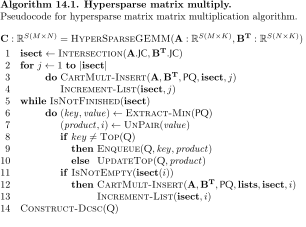
\includegraphics{hypersparseMM.svg.png}
  \caption[Algoritmo sequenziale per SpMM tra matrici ipersparse] \decoRule \label{figCode:hypersparseMM}
\end{figure}

\begin{figure}[h!]
  \centering 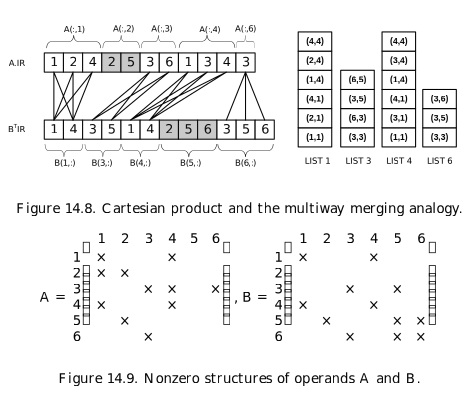
\includegraphics{hypersparseMMGraphical.svg.png}
  \caption[Rappresentazione grafica del prodotto cartesiano 
   a supporto di hypersparseMM ] \decoRule \label{fig:hypersparseMMGraphical}
\end{figure}


\subsection{Algoritmi con un partizionamento 2D}

\subsubsection{Derivati di Gustavson} \label{ssec:gustavsonDerivate}
Una parallelizzazione della formulazione per righe dell'algoritmo di Gustavson è
descritta in \cite{intelSpMMDenseAccumulator}, sfruttando la
rappresentazione di matrici sparse in formato CSR.  \label{ssec:intelSpMMDenseAccumulator}
Lo pseudocodice dell'algoritmo è riportato in \ref{figCode:gustavsonRigheBlocksIntel}
e una sua rappresentazione grafica è raffigurata in
\ref{fig:gustavsonRigheBlocksGraphicalIntel}\\
%Partizionamento = Gustvason a blocchi
Viene effettuato un partizionamento delle righe di A e delle colonne di B e 
coppie di partizioni corrispondenti vengono utilizzate per calcolare un
blocco bidimensionale della matrice risultante C.\\
%accumulatore denso X
In accordo con la formulazione per righe dell'algoritmo di Gustavson, vengono
accumulati i contributi degli elementi \nnz delle righe di A e corrispettive porzioni
delle righe di B relative al calcolo di un blocco di C. 
Per effettuare efficientemente questa operazione, i vettori sparsi risultanti
dalle iterazioni dell'algoritmo, vengono accumulati in vettore denso X, 
semplicemente sommandone le componenti \nnz nelle relative locazioni di X.\\
%alternative memory efficient con overhead
In questa formulazione del problema, una soluzione di accumulazione 
alternativa potrebbe essere quella di accumulare i contributi per una riga di C 
utilizzando una hash-table di elementi aventi per chiave l'indice di colonna. 
Tuttavia, quest'approccio ha lo svantaggio di avere l'overhead relativo alla 
computazione delle funzioni hash e gestione di eventuali liste di collisione.\\
%implementazione conversione
Al termine del calcolo di una riga di un blocco di C, l'accumulare X viene
convertito in una riga CSR con l'ausilio di un ulteriore vettore di indici di
elementi \nnz sommati in X.\\
%Nota su partizionamento -> MENO cache miss su X
Utilizzando un partizionamento delle colonne di B è possibile partizionare anche
l'accumulatore X relativo ad una riga risultante di C. In questa maniera si
riduce il numero di cache line toccate dagli aggiornamenti di X, riducendo il
numero di cache miss relativi al ciclo interno dell'algoritmo.\\
Gli autori dell'algoritmo hanno verificato la riduzione di cache miss
utilizzando degli hardware counter per verificare il numero di cache miss L2
(tipicamente catturati dalla cache LLC) al variare del partizionamento di B % TODO QUANTIFICAZIONE?
%%Valutazione sul partizionamento di B -> X
%svantaggi
Tuttavia il partizionamento di B in rappresentazioni CSR separate, 
oltre che comportare un overhead computazionale, può comportare svantaggi in
termini di banda di memoria durante la lettura dei blocchi di B, che possono
essere notevolmente più sparsi della matrice originaria. %TODO link a ipersparse
%quantificazione euristica beneficio
Un beneficio dal partizionamento di B e di X, contro gli overhead citati, è
presente quando si ha certezza che per una significativa porzione delle righe
risultanti di C, l'occupazione dei non zeri, corrispondenti agli aggiornamenti
dell'accumulatore X, è maggiore della dimensione della cache L2.\\
Per quantificare il numero di \nnz nelle righe risultanti di C viene utilizzata
una metrica basata sulla stima di \nnz in $c_{i*}=e\_nnz(i)$ di
\cite{intelSpMMDenseAccumulator} %TODO SOURCE ARTICLE OF ESTIMATE
dove si partiziona B se
$e\_nnz = \frac{\sum\limits_{i:e\_nnz(i) > L2\_FP\_WORDS} e\_nnz(i)}
{\sum\limits_{i=1}^m e\_nnz(i)} ~>~0.3$\\
%TODO scheduling dinamico -> load balancing con perizioni piccole t.c. #partizioni = 6-10 X #threads
\begin{figure}[h!]
  \centering \includegraphics{gustavsonRigheBlocksIntel.svg.png}
  \caption[adattamento parallelo dell'algoritmo di Gustavson] \decoRule \label{figCode:gustavsonRigheBlocksIntel}
\end{figure}
\begin{figure}[h!]
  \caption[rappresentazione grafica dell'adattamento parallelo dell'algoritmo di Gustavson] 
  \centering \includegraphics{gustavsonRigheBlocksGraphicalIntel.svg.png} \label{fig:gustavsonRigheBlocksGraphicalIntel}
\end{figure}

L'uso di un vettore denso per operazioni tra matrici sparse è stato 
affrontato originariamente da \cite{SPA_mathlab}.\\

\subsubsection{Dense SUMMA} %versione base C=AB
Un partizionamento bidimensionale della risoluzione del prodotto tra matrici
dense è realizzato dell'algoritmo parallelo SUMMA \cite{denseSumma} che è alla
base di una sua controparte per matrici sparse \cite{sparseSUMMA}.\\
Il calcolo di $C=AB$ è suddiviso in sottomatrici assegnate a processi organizzati 
in una griglia bidimensionale di dimensione  $p_r x p_c$.\\
È possibile calcolare un blocco della matrice C come:
$C_{ij} =  \overbrace{\left(  A_{i1} | \dots |  A_{ip_c} \right)}^{\tilde{A^{i*}} }
~\cdot~ \overbrace{\left( 
        \begin{array}{c} B_{1j} \\ \vdots \\  B_{p_r j}
        \end{array} \right)} ^{\tilde{B^{*j}}} $\\
dove si usa la notazione:
\begin{itemize}
  \item $\tilde{a_{*l}}^{i*} \in \tilde{ A^{i*}}$ rappresenta 
    la colonna l-esima nella riga i-esima nella decomposizione a blocchi di A
  \item $\tilde{b_{l*}}^{*j} \in  \tilde{B^{*j}}$ rappresenta 
    la riga l-esima nella colonna j-esima nella decomposizione a blocchi di B.
\end{itemize}  
Applicando la formulazione outer-product su $\tilde{ A^{i*}}$ e $\tilde{B^{*j}}$
si ha che $C_{ij}=\sum\limits_{l=1}^{k}\tilde{a_{*l}}^{i*} \cdot \tilde{b_{l*}}^{*j}$\\
Considerando un partizionamento delle matrici in sottomatrici all'interno della
griglia di processi %assegnate in maniera tale che  ... 
si può eseguire l'operazione MM in parallelo come riportato dallo pseudocodice
in \ref{figCode:denseSUMMA}\\
\begin{figure}[h!]
  \centering 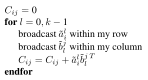
\includegraphics{denseSUMMA.svg.png}
  \caption[esecuzione dense SUMMA sul processo $P_{ij}$] \decoRule \label{figCode:denseSUMMA}
\end{figure}
Nell'articolo originale vengono discussi miglioramenti a questa formulazione
basati su uno scambio di dati tra i processi in un sistema a memoria distribuita
mediante una comunicazione ad anello 
riformulazione del calcolo di $C_{ij}$ utilizzando blocchi di
colonne di $\tilde{ A^{i*}}$ e righe di $\tilde{B^{*j}}$.\\

\subsubsection{Sparse SUMMA}
Un partizionamento bidimensionale del problema SpMM è realizzato
dall'algoritmo Sparse SUMMA \cite{sparseSUMMA}, derivato dalla sua
controparte per matrici dense.\\
%SPARSE SUMMA
È riportato lo pseudo-codice dell'algoritmo sparseSUMMA 
in \ref{figCode:sparseSUMMA} e una sua iterazione graficamente in
\ref{fig:sparseSUMMAIteration}.\\
Le matrici sono divise in blocchi e rappresentante in formato DCSC,
trasponendo la matrice B per avere un indicizzamento rapido delle sue righe.\\
Procedendo in blocchi di colonne di una sottomatrice di A e della corrispettiva
sottomatrice di $B^T$, lungo la dimensione comune di A e B,
vengono calcolati in parallelo le sottomatrici $C_{ij}$, 
utilizzando l'algoritmo hypersparseMM \ref{ssec:hypersparseMM}.\\
Il costo computazionale dell'algoritmo è 
$O(\frac{dn}{\sqrt{p}}+\frac{d^2n}{p}lg(\frac{d^2n}{p}))$
%TODO CONSIDERAZIONE SU EFFICIENZA ALLO SCALARE DI p ... cmq no speedup bounds!
\begin{figure}[h!]
  \caption[SparseSUMMA, per una risoluzione parallela di SpMM con un partizionamento 2D]
  \centering \includegraphics{sparseSUMMA.svg.png} \decoRule \label{figCode:sparseSUMMA}
\end{figure}
\begin{figure}[h!]
  \caption[esecuzione di un iterazione dell'algoritmo sparseSUMMA]
  \centering \includegraphics{sparseSUMMAIteration.svg.png} \decoRule \label{fig:sparseSUMMAIteration}
\end{figure}

\subsection{Algoritmi con un partizionamento 3D}
Un partizionamento tridimensionale del problema SpMM è realizzato dall'
algoritmo Split-3D-SpMM \cite{Split3DSpMM}, dove al partizionamento
bidimensionale descritto precedentemente, viene aggiunto una ulteriore
suddivisione delle sottomatrici in blocchi nella terza dimensione della griglia di processi.
%TODO CONSIDERAZIONI su overhead mem per C -> sparsity-structure dependent ->
%sfruttabile bene la sparsità del risultato in meno occupazione di memoria
Il partizionamento delle matrici è rappresentabile sul cubo di lavoro W come
riportato in figura \ref{fig:workCube3D}, dove il processo P(i,j,k) possiede la
porzione della matrice di A: 
$A(im/p_r:(i+1)m/p_r - 1, jn/p_c + kn/(p_c p_l ) : jn/p_c + (k + 1)n/(p_c p_l) - 1)$  \\
\begin{figure}[h!]
  \caption[rappresentazione 3D della suddivisione della computazione SpMM]
  \centering \includegraphics{workCube3D.svg.png} \decoRule \label{fig:workCube3D}
\end{figure}
L'algoritmo è riportato nello pseudo-codice \ref{figCode:Split3DSpMM} e una
sua iterazione è raffigurata graficamente in \ref{fig:Split3DSpMMIteration}.\\

In maniera simile al caso di sparseSUMMA %TODO \ref{sparseSummaDescriptionStart}
si procede in parallelo calcolando il prodotto di sotto blocchi corrispondenti
alle sottomatrici di A e B, accumulando risultati intermedi la cui collocazione
è relativa all'intera fiber W(i,j,:).
Infine i risultati intermedi dei processi P(i,j,:), vengono distribuiti lungo la fiber
W(i,j,:), sommando i contributi relativi agli stessi indici.
\begin{figure}[h!] 
  \caption[Split3DSpMM, per una risoluzione parallela di SpMM con un partizionamento 3D
     nel caso semplificato di una griglia di processi $\sqrt{p/c}~x~\sqrt{p/c}~x~c$]
  \centering 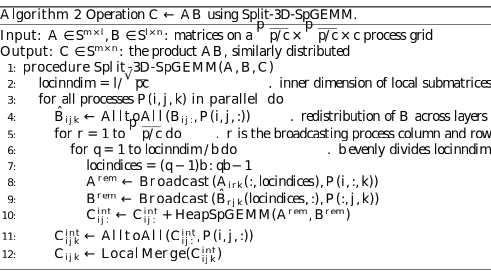
\includegraphics[width=1.0\textwidth]{Split3DSpMM.svg.png} \decoRule \label{figCode:Split3DSpMM}
\end{figure}
\begin{figure}[h!]
  \caption[esecuzione di un iterazione dell'algoritmo Split3DSpMM]
  \centering \includegraphics[width=1.0\textwidth]{Split3DSpMMIteration.svg.png} 
  \decoRule \label{fig:Split3DSpMMIteration}
\end{figure}

\section{Algoritmi paralleli basati su formulazione Outer-Product}
%\item Outer-product \qquad $C = \sum\limits_{i=1}^k  a_{*i} \otimes  b_{i*}$		
Implementazioni di SpMM basate su formulazioni di Outer-Product, godono di una
potenziale migliore località spaziale dei \nnz acceduti durante il prodotto,
come spiegato in \cite{ESC}.\\
\label{ChExistingTecqs:gustavsonDerivateBadAccessLocalityNNDominantMatrix}
Considerando rispettivamente formulazioni row-by-row e col-by-col per SpMM e denominando 
la matrice dominante nei prodotti rispettivamente A e B,
si ha una buona località spaziale per le matrici dominanti e risultanti ma non per quelle non dominanti.
Questo è dovuto al fatto che la matrice non dominante deve essere acceduta per righe o colonne 
in un ordine derivato dal pattern di sparsità dei non zeri delle matrici dominanti, che è assimilabile ad un ordine casuale.\\

Nel caso row-by-row ad esempio, si può avere un cattivo uso della cache in scenari dove:\\
una riga di B deve essere riletta varie volte, ma l'ordinamento degli accessi alle righe di B causa
che, il più delle volte, la riga non sia in cache quando necessario.\\
In questi casi si ha che formulazioni row-by-row o col-by-col causano uno spreco di banda di memoria,
il che è particolarmente critico per un problema memory bound come SpMM.\\
%%OuterProduct visual
\begin{figure}[h!]
  \centering 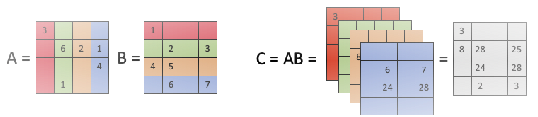
\includegraphics{imgs/outerProductExampleVisual_ESC.svg.png}
  \caption[Visualizzazione di un prodotto tra matrici 4x4 mediante Outer-Product]
  \decoRule \label{fig:outerProductExampleVisual_ESC}
\end{figure}

\subsection{ESC - PropagationBlocking}
Una soluzione per l'operazione di SpMM mediante Outer-Product è riportata in \cite{ESC},
dove viene usato un algoritmo basato sul generale approccio risolutivo Expand-Sort-Compress, %TODO cerca di piu ESC in generale
applicato ad una formulazione Outer-Product per SpMM.\\

Le principali fasi dell'algoritmo sono:
\begin{itemize}
	\item $\hat{C}~\leftarrow~$Symbolic(A,B) \\ Allocazione dei risultati intermedi al prodotto mediante un UpperBound
	\item $\hat{C}~\leftarrow~$Expand(A,B)	 \\ Esecuzione dei prodotti a rango 1 della formulazione Outer-Product in formato COO
	\item Sort($\hat{C}$) 					 \\ Ordinamento mediante radix-sort dei prodotti intermedi mediante le loro coordinate risultanti
	\item $C~\leftarrow~$Compress($\hat{C}$) \\ unione dei risultati intermedi, sommandoli nella matrice finale
\end{itemize}

%%Algo Steps bigPic
\begin{figure}[h!]
  \centering 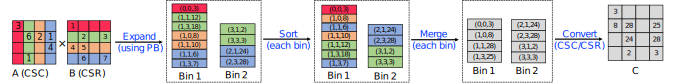
\includegraphics{OuterProduct_PBAlgoritmExample_ESC.svg.png}
  \caption[Rappresentazione grafica degli step principali dell'algoritmo] 
  \decoRule \label{fig:OuterProduct_PBAlgoritmExample_ESC}
\end{figure}

\subsubsection{Symbolic -- UB estimate}
Analogamente a quanto descritto precedentemente in \ref{ChExistingTecqs:openMP_for_philosophy}, 
preferendo una preallocazione delle strutture intermedie necessarie rispetto ad effettuare (ri)allocazioni dinamiche, 
viene calcolata la dimensione dei risultati intermedi che corrisponde ad un UpperBound della dimensione finale del risultato.\\
Seguendo un approccio Outer-Product per SpMM, il numero di \nnz al termine della fase Expand è pari ad:\\
$ \sum\limits_{i = 1}^k  | I^i(A) | *| I_i(B) | $ \\ % flops + = nnz(B(i, :)) × nnz(A(:, i))
 
\subsubsection{Expand}
In questa fase vengono effettuati i prodotti richiesti dalla formulazione Outer-Product, 
salvando i non zeri come tuple con il risultato numerico e le coordinate di righe e colonne (formato COO).\\
Per questioni di efficienza è necessario che la matrice A sia in un formato con colonne contigue (CSC) 
e B in un formato con righe contigue (CSR).\\
Queste tuple vengono generate e raggruppate in parallelo in bin in base agl'indici di riga dei corrispondenti elementi di A.\\
Per una maggiore efficienza ogni thread mantiene una copia locale di tutti i $m$ bin possibili, 
effettuando periodicamente una operazione di \emph{flush} dei dati locali nei bin globali.\\ 

\begin{figure}[h!]
  \centering 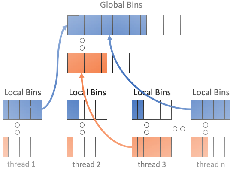
\includegraphics{OuterProduct_PBAlgo_BinsExample_ESC.svg.png}
  \caption[Rappresentazione grafica delle operazioni di flush periodiche dei bin locali ai thread nei bin globali]
  \decoRule \label{fig:OuterProduct_PBAlgo_BinsExample_ESC.svg.png}
\end{figure}

%PropagationBlocking Explaination ... TODO non menzionato esplicitamente nel paper... interpolato da qua e la xD
Il termine "PropagationBlocking" deriva da questa organizzazione dei prodotti in Bin locali e globali, 
consentendo insieme alle fasi successive una somma efficiente dei valori 
corrispondenti allo stesso elemento \nnz nella matrice risultante.\\

\subsubsection{Sort}
Si effettua un sorting delle tuple prodotte in $\hat{C}$ nei bin globali nella fase precedente,
ordinandole in base ai campi relativi alle coordinate di righe e colonne.\\
Gli autori dell'articolo asseriscono di usare una versione inplace di radix-sort, 
che raggruppa le chiavi in base alla posizione del byte più significativo 
(richiedendo cosi un numero di passate sui dati proporzionale al numero di byte nelle chiavi),
dando performance migliori rispetto ad algoritmi basati su comparazioni per chiavi piccole.\\
Utilizzando un numero di bin tale da averene la maggior parte in dimensione tale 
da poter entrare in cache L2 o L3 è possibile effettuare il sorting in cache, 
attenuando il costo dovuto alle riletture dei dati per l'operazione di ordinamento.

\subsubsection{Compress}
Si sommano tutte le tuple aventi stesse cordinate di riga e colonna, corrispondenti allo stesso elemento non zero
nella matrice risultante.\\
Grazie all'ordinamento effettuato nella fase precedente, è possibile completare questa fase con una singola
scansione di tutti i Bin globali.\\


Per facilitare le fasi di Sort e Compress, il numero di bin globali può essere determinato nella fase simbolica 
dividendo il numero di tuple attese per la dimensione della cache L2 del dispositivo di calcolo.
Questo consente che i bin globali nelle ultime 2 fasi possano entrare in cache L2, 
migliorando l'utilizzo della memoria durante l'esecuzione in parallelo.\\









%%Figure options
%%h 	Place the float here, i.e., approximately at the same point it occurs in the source text (however, not exactly at the spot)
%%t 	Position at the top of the page.
%%b 	Position at the bottom of the page.
%%p 	Put on a special page for floats only.
%%! 	Override internal parameters LaTeX uses for determining "good" float positions.
%%H 	Places the float at precisely the location in the LaTeX code. Requires the float package, though may cause problems occasionally. This is somewhat equivalent to h!.
